\documentclass{beamer}
\usepackage{stmaryrd}
\usepackage{amsthm}
\usepackage{amssymb}
\usepackage{amsmath}
\usepackage{algorithm2e}
\usepackage{hyperref}
\usepackage[french]{babel}
\usepackage{color}
\usepackage{tikz}
\usetikzlibrary{automata, arrows.meta, positioning}
\usepackage{MacrosBeam}

%% Generated by ipescript page-labels figs.pdf
%% Do not edit
\newcommand{\ipeFigexcarte}{1}
\newcommand{\ipeFigKKnIpqcompl}{2}
\newcommand{\ipeFigcartetrivperf}{3}
\newcommand{\ipeFigextrivperf}{4}
\newcommand{\ipeFigIpqIrsMap}{5}
\newcommand{\ipeFigIpqIrsItuMap}{6}
\newcommand{\ipeFigtemoinK}{7}
\newcommand{\ipeFigpointabuse}{8}
\newcommand{\ipeFigcographsepind}{9}
\newcommand{\ipeFigfirsttemoin}{10}
\newcommand{\ipeFigfirsttemoinquatriparti}{11}
\newcommand{\ipeFigsecondtemoinquatriparti}{12}
\newcommand{\ipeFigpinch}{13}
\newcommand{\ipeFigTemoinAbsurde}{14}
\newcommand{\ipeFigtrivPerftriconn}{15}
\newcommand{\ipeFigtypicalmaptrivperf}{16}
\newcommand{\ipeFigdecomptriconnOne}{17}
\newcommand{\ipeFigdecomptriconnTwo}{18}
\newcommand{\ipeFigdecomptriconnThree}{19}
\newcommand{\ipeFigjoinex}{20}
\newcommand{\ipeFiguniondisjex}{21}

\usetheme{Boadilla}
\usecolortheme{seahorse}

\title{Reconnaissance et caractérisations partielles des graphes de carte}

\author{José Lorgeré}

\institute{Encadré par Vincent Limouzy}

\begin{document}

\frame{\titlepage}

\begin{frame}
    \frametitle{Table des matières}

    \tableofcontents

\end{frame}

\AtBeginSection[ ]
{
    \begin{frame}{Table des matières}
        \tableofcontents[currentsection]
    \end{frame}
}

\section{Résultats précédents sur la reconnaissance des graphes de carte}

\begin{frame}{Définitions}

    \begin{definition}[Graphe de carte]
        Soit $G = (V, E)$ un graphe. S'il existe une fonction $f$ de $V$ dans les parties de la sphère $\mathbb{S}^2$ vérifiant que
        \begin{itemize}
            \item Pour tout $v \in V$, $f(v)$ est homéomorphe au disque $\mathbb{D}^2$
            \item Les intérieurs des $f(v)$ sont disjoints
            \item On a $uv \in E$ si et seulement si $f(v)$ et $f(u)$ se rencontrent
        \end{itemize}
        On dira que $G$ est un graphe de carte, que $f$ est une carte de $G$, et on appelera les $f(v)$ régions.
        Si $f$ forme un recouvrement de la sphère, on dira que $f$ est complète.
    \end{definition}

\end{frame}

\begin{frame}
    
    \begin{figure}
        \caption{Un graphe, et une carte de ce dernier}

        \begin{tikzpicture}[auto]
            \begin{scope}[every node/.style={circle, draw}]

            \node (a) {$a$};
            \node (h) [left = of a] {$h$};
            \node (e) [right = of a] {$e$};
            \node (b) [below = of h] {$b$};
            \node (g) [below = of b] {$g$};
            \node (c) [right = of g] {$c$};
            \node (d) [below = of e] {$d$};
            \node (f) [below = of d] {$f$};
            \end{scope}

            \path
            (a) edge (b) edge (c) edge (d) edge (e) edge (h)
            (b) edge (c) edge (d) edge (h) edge (g)
            (c) edge (d) edge (g) edge (f)
            (d) edge (e) edge (f);
        \end{tikzpicture}
        \hspace*{1cm}
        \includegraphics[page=\ipeFigexcarte, scale = 0.5]{figs}
    \end{figure}

\end{frame}

\begin{frame}{Caractérisation}
    \begin{thm}[Chen, Grigni, Papadimitriou, 2002]
        Un graphe $G = (V, E)$ est de carte si et seulement il existe un graphe planaire biparti $H$ de bipartition $V, U$
        tel que $H^2[V] = G$. Un tel graphe $H$ sera appelé un témoin de $G$.
    \end{thm}

    On peut alors voir que la classe des graphes planaires est sous classe stricte des graphes de carte.
\end{frame}

\begin{frame}
    \begin{figure}
        \caption{Un graphe et son témoin}

        \begin{tikzpicture}[auto]
            \begin{scope}[every node/.style={circle, draw}]

            \node (a) {$a$};
            \node (h) [left = of a] {$h$};
            \node (e) [right = of a] {$e$};
            \node (b) [below = of h] {$b$};
            \node (g) [below = of b] {$g$};
            \node (c) [right = of g] {$c$};
            \node (d) [below = of e] {$d$};
            \node (f) [below = of d] {$f$};
            \end{scope}

            \path
            (a) edge (b) edge (c) edge (d) edge (e) edge (h)
            (b) edge (c) edge (d) edge (h) edge (g)
            (c) edge (d) edge (g) edge (f)
            (d) edge (e) edge (f);
        \end{tikzpicture}
        \hspace*{1cm}
        \includegraphics[page=\ipeFigfirsttemoin, scale = 0.38]{figs}
    \end{figure}
\end{frame}

\begin{frame}{Quelques propriétés}
    \begin{proposition}
        Soit $G = (V, E)$ un graphe de carte, $S \subset V$. $G[S]$ est également de carte
    \end{proposition}

    Les graphes de carte ne sont toutefois pas stables par retrait d'arrête ni par contraction d'arrêtes comme on
    le verra ensuite.

    \begin{proposition}
        Un graphe $G$ est de carte si et seulement si ses composantes $2$-connexes sont de carte.
    \end{proposition}

    On considèrera par la suite tout les graphes étudiés $2$-connexes.
\end{frame}

\begin{frame}{Reconnaissance}
    Le problème de reconnaissance des graphes de carte est dans NP (Chen, Grigni, Papdimitriou, 2002).

    \begin{conj}[Chen, Grigni, Papadimitriou, 2002]
        Le problème de reconnaissance des graphes de carte peut être résolu en temps polynômial.
    \end{conj}

    Thorup publie en 1998 un algorithme reconnaissant en temps polynômial (éstimé $O(n^{120})$) les graphes
    de carte. Les détails ne sont toutefois jamais publiés
\end{frame}

\begin{frame}{Quelques résultats prometteurs}
    \begin{thm}[Chen, Grigni, Papadimitriou, 2002]
        Le problème de reconaissance, restreint aux graphes admettant une carte complète et tel que chaque point
        de la sphère est dans au plus $4$ régions distinctes, peut être résolu en temps polynômial
    \end{thm}

    \begin{thm}[Angelin, Bekos, Da Lozzo, Gronemann, Montecchiani, Tappini, 2024]
        Le problème de reconnaissance paramétré par la largeur d'arbre est FPT
    \end{thm}
\end{frame}

\section{Recherche de petits graphes sans carte}

\begin{frame}{Définitions}
    \begin{definition}[Join et union disjointe]
        Le join de deux graphes $G = (V, E)$, $G' = (V', E')$ est le graphe sur les sommets $V \cup V'$ tel
        que les arrêtes entre sommets de $V$ soient conservées identiques, de même entre ceux de $V'$. Toutefois,
        chaque sommet de $V$ est adjacent à tout ceux de $V'$ et inversement. On notera ce graphe $K(G, G')$.
        \\~\\
        On définit l'union disjointe de manière similaire, à la différence près que les sommets de $V$ et $V'$ sont
        indépendants, et on note le graphe obtenu $I(G, G')$.
    \end{definition}
\end{frame}

\begin{frame}
    \begin{figure}
        \caption{Le join et l'union disjointe de deux graphes}
        \includegraphics[page=\ipeFigjoinex, scale = 0.7]{figs}
        \hspace*{1cm}
        \includegraphics[page=\ipeFiguniondisjex, scale = 0.7]{figs}
    \end{figure}
\end{frame}

\begin{frame}{Notations}
    On notera le join d'un indépendant à $n$ sommets avec un graphe $G$, $K(n, G)$.
    \\~\\
    On notera l'union disjointe d'un graphe complet à $n$ sommets avec un graphe $G$, $I(n, G)$. On désignera aussi
    par $I_{n_1, ..., n_k}$ l'union disjointe des cliques à $n_1, ...,  n_k$ sommets
\end{frame}

\begin{frame}
    \begin{thm}[Wagner, 1937]
        Un graphe $G$ est planaire si et seulement s'il ne possède pas de mineurs $K_5$ ou $K_{3,3}$.
    \end{thm}

    On en déduit le résultat suivant :

    \begin{proposition}
        Pour tout graphe $G$ a $3$ sommets, $K(3, G)$ n'est pas de carte.
    \end{proposition}
\end{frame}

\begin{frame}{Démonstration}
    On suppose par l'absurde que $K(3, G)$ est de carte. On considère un témoin de ce dernier, $H$.
    \begin{figure}
        \begin{center}
            \includegraphics[page=\ipeFigTemoinAbsurde, scale = 0.5]{figs.pdf}
        \end{center}
    \end{figure}
    Ce dernier contient nécessairement un mineur $K_{3,3}$.
\end{frame}

\begin{frame}{Autres graphes interdits}
    \begin{proposition}
        Les graphes suivants ne sont pas de carte :
        \begin{itemize}
            \item $K_{2,2,2,2,1}$
            \item $K(2,2,2,I_{2,1})$
            \item $K(2,2,2,K_5)$
        \end{itemize}
    \end{proposition}

    On utilise en plus des mineurs interdits d'autres méthodes spécifiques aux graphes étudiés $K(2,2,2,...)$
\end{frame}

\begin{frame}
    On déduit de l'existence de ces graphes sans carte que les graphes de carte ne sont pas stables par retrait
    d'arrête (les graphes complets sont de carte). Ils ne le sont également pas par contraction d'arrête

    \begin{figure}
    \caption{Un graphe de carte dont la contraction de $xy$ le transforme en un $K(3, G)$.}\label{nonstabcontrarr}
    \vspace*{0.5cm}
    \begin{center}
        \includegraphics[page=\ipeFigpinch, scale = 0.6]{figs}
    \end{center}
\end{figure}
\end{frame}

\section{Etudes de sous classes de graphes de carte}

\subsection{Graphes trivialement parfaits de carte}

\begin{frame}{Définition}
    Un graphe trivialement parfait est un graphe sans $P_4, C_4$ induits. De manière équivalente, il peut être
    représenté par l'intersection d'intervalles emboîtés

    \begin{figure}
    \caption{Un graphe trivialement parfait représenté par des intervalles emboîtés.}
    \begin{center}
    \includegraphics[page=\ipeFigextrivperf, scale = 0.85]{figs}
    \end{center}
\end{figure}
\end{frame}

\begin{frame}{Stratégie générale}
    On souhaite caractériser les graphes de carte trivialement parfaits. On procèdera ainsi :
    \begin{itemize}
        \item On caractérisera les graphes trivialement parfaits $3$-connexes
        \item On utilisera ces résultats pour en déduire le cas général $2$-connexe
    \end{itemize}
\end{frame}

\begin{frame}{Caractérisation}
    \begin{proposition}
        Un graphe trivialement parfait $3$-connexe $G$ est de carte si et seulement si il s'agit
        d'un $K_n$ ou d'un $K(I_{p,q}, K_n)$, $n \geq 3$.
    \end{proposition}

    On aura besoin du lemme suivant

    \begin{lem}
        Un graphe trivialement parfait $3$-connexe de carte ne peut avoir un indépendant de taille $3$.
    \end{lem}
\end{frame}

\begin{frame}{Preuve du lemme}
    \begin{figure}
        \caption{Un graphe trivialement parfait $3$-connexe possédant $3$ sommets indépendants}
        \begin{center}
            \includegraphics[page=\ipeFigtrivPerftriconn, scale = 0.75]{figs}
        \end{center}  
    \end{figure}

    Si il existait un indépendant de taille $3$, en considérant cet ensemble et $3$ universels du graphe,
    on construit un sous graphe induit $K(3, K_3)$.
\end{frame}

\begin{frame}{Preuve de la proposition, sens direct}
    Si $G$ est de carte et n'est pas une clique,
    le lemme assure que le graphe est de la forme suivante, où $U_1$ et $U_2$ sont des cliques, tout comme $U$.

    \begin{figure}
        \begin{center}
            \includegraphics[page=\ipeFigtypicalmaptrivperf, scale = 0.75]{figs}
        \end{center}
    \end{figure}
\end{frame}

\begin{frame}{Preuve de la proposition, sens réciproque}
    Si $G$ est une clique, il est de carte. Sinon, $G$ est un $K(K_n, I_{p,q})$ :

    \begin{figure}[h]
    \caption{Carte de $K(K_n, I_{p,q})$.}
    \begin{center}
        \includegraphics[page=\ipeFigKKnIpqcompl, scale = 0.4]{figs}
    \end{center}
\end{figure}
\end{frame}

\begin{frame}{Décomposition $3$-connexe}
    On considère un graphe $2$-connexe $G$ possédant un séparateur de taille $2$, $\{x,y\}$.

    \begin{figure}
        \begin{center}
            \includegraphics[page=\ipeFigdecomptriconnOne, scale = 0.6]{figs}
        \end{center}
    \end{figure}
\end{frame}

\begin{frame}{Décomposition $3$-connexe}
    On considère un graphe $2$-connexe $G$ possédant un séparateur de taille $2$, $\{x,y\}$.

    \begin{figure}
        \begin{center}
            \includegraphics[page=\ipeFigdecomptriconnTwo, scale = 0.6]{figs}
        \end{center}
    \end{figure}
\end{frame}

\begin{frame}{Décomposition $3$-connexe}
    On considère un graphe $2$-connexe $G$ possédant un séparateur de taille $2$, $\{x,y\}$.

    \begin{figure}
        \begin{center}
            \includegraphics[page=\ipeFigdecomptriconnThree, scale = 0.6]{figs}
        \end{center}
    \end{figure}
\end{frame}

\begin{frame}{Décomposition $3$-connexe}
    On appelle composantes $3$-connexes de $G$ associées à une décomposition les graphes $3$-connexes obtenus
    après répétition du processus, où le choix du séparateur est spécifié par la décomposition.
    \\~\\
    Toutefois, pour les graphes trivialement parfaits, la décomposition est unique (il n'y a qu'un seul séparateur
    de taille $2$, et qu'une seule étape de décomposition). On dispose également du résultat suivant

    \begin{proposition}
        Soit $G$ un graphe de carte $2$-connexe. Ses composantes $3$-connexes sont de carte pour toute décomposition
        choisie.
    \end{proposition}
\end{frame}

\begin{frame}{Cas général $2$-connexe}
    \begin{thm}
        Soit $G$ un graphe trivialement parfait $2$-connexe. Ce dernier est de carte si et seulement si toutes ses
        composantes $3$-connexes le sont.
    \end{thm}

    \begin{proof}
        Le sens direct est déjà fait. Le sens réciproque utilise la forme des composantes $3$-connexes d'un
        graphe de carte trivialement parfait.
    \end{proof}
\end{frame}

\begin{frame}
    \begin{figure}
        \caption{Un exemple de carte d'un graphe de carte trivialement parfait $2$-connexe}
        \begin{figure}
            \includegraphics[page=\ipeFigcartetrivperf, scale = 0.45]{figs}
        \end{figure}
    \end{figure}
\end{frame}

\subsection{Cographes de carte}

\begin{frame}{Table des matières}
    \tableofcontents[currentsection, currentsubsection]
\end{frame}

\begin{frame}{Définitions}
    Un cographe est un graphe que l'on peut construire uniquement grâce aux opération de join
    et d'union disjointe ($K$ et $I$) (soit sans $P_4$ induit).

    \begin{figure}
        \caption{Le cographe $K(2, I(1, K_{2,2}))$}
        \begin{center}
        \begin{tikzpicture}[auto]
            \begin{scope}[every node/.style={circle, draw}]
                \node (1) {$v_1$};
                \node (2) [left = of 1] {$v_2$};
                \node (3) [below left = of 2] {$v_3$};
                \node (4) [below = of 3] {$v_4$};
                \node (5) [below right = of 4] {$v_5$};
                \node (6) [right = of 5] {$v_6$};
                \node (a) [below left = 4mm and 10mm of 3] {$a$};
            \end{scope}

            \path
            (1) edge (3) edge (4) edge (5) edge (6)
            (2) edge (3) edge (4) edge (5) edge (6)
            (a) edge (3) edge (4)
            (3) edge (5) edge (6)
            (4) edge (5) edge (6);
        \end{tikzpicture}
    \end{center}
    \end{figure}

\end{frame}

\begin{frame}{Coarbre}
    En représentant les opérations $K$ et $I$ par un arbre et en "compactant" ce dernier on obtient pour tout cographe
    une représentation unique par un "coarbre"

    \begin{figure}
        \caption{Le coarbre de $K(2, I(1, K_{2,2}))$}
        \begin{center}
        \begin{tikzpicture}[auto]
            \begin{scope}[every node/.style={circle, draw}]
                \node (0) {$1$};
                \node (00) [below left = 7mm and 15mm of 0] {$0$};
                \node (01) [below right = 7mm and 15mm of 0] {$0$};
                \node (000) [below left = 7mm and 7mm of 00] {$1$};
                \node (001) [below right = 7mm and 7mm of 00] {$a$};
                \node (010) [below left = 7mm and 7mm of 01] {$v_3$};
                \node (011) [below right = 7mm and 7mm of 01] {$v_4$};
                \node (0000) [below left = 7mm and 7mm of 000] {$0$};
                \node (0001) [below right = 7mm and 7mm of 000] {$0$};
                \node (00000) [below left = 5mm and 1mm of 0000] {$v_1$};
                \node (00001) [below right = 5mm and 1mm of 0000] {$v_2$};
                \node (00010) [below left = 5mm and 1mm of 0001] {$v_5$};
                \node (00011) [below right = 5mm and 1mm of 0001] {$v_6$};
            \end{scope}

            \path
            (0) edge (00) edge (01)
            (00) edge (000) edge (001)
            (000) edge (0000) edge (0001)
            (0000) edge (00000) edge (00001)
            (0001) edge (00010) edge (00011)
            (01) edge (010) edge (011);

        \end{tikzpicture}
    \end{center}
    \end{figure}
\end{frame}

\begin{frame}{Caractérisation $3$-connexe}
    \begin{thm}
        Soit $G$ un cographe $3$-connexe. $G$ est de carte si et seulement si il est de l'une des formes suivantes
        \begin{itemize}
            \item $K_n$, $n \geq 3$
            \item $K(I_{p,q}, K_n)$, $n \geq 3$
            \item $K(I_{p,q}, I_{r,s}, K_n)$, $p,q,r,s \geq 1$, $n \geq 0$, tels que le graphe soit $3$-connexe
            \item $K(I_{p,q}, I_{r,s}, I_{t,u}, K_n)$, $p,q,r,s,t,u \geq 1$, $n \leq 4$
            \item $K_{2,2,2,2}$
        \end{itemize}
    \end{thm}

    La démonstration utilise les sous graphes interdits $K(3,H), K_{2,2,2,2,1}, K(2,2,2,I_{2,1}), K(2,2,2,K_5)$
    pour contraindre le coarbre de $G$.
\end{frame}

\begin{frame}{Type}
    \begin{definition}
        Un cographe de carte $3$-connexe sera dit de type $0, 1, 2, 3, 4$ selon la taille de son indépendant
        maximum.
    \end{definition}
    Chaque type correspond en fait à une des formes décrites précédemment, dans l'ordre.
\end{frame}

\begin{frame}{Caractérisation strictement $2$-connexe}
    On peut montrer que tout cographe a plus de $5$ sommets a une unique décomposition $3$-connexe.

    \begin{thm}
        Soit $G$ un cographe $2$-connexe à plus de $5$ sommets et $\{x,y\}$ un séparateur minimal de $G$. 
        \begin{itemize}
            \item Si $xy \in E$, $G$ est de carte si et seulement si toutes ses composantes $3$-connexes sont de carte de type au plus $2$.
            \item Sinon, $G$ est de carte si et seulement si chaque composante $3$-connexe de $G$ est de carte de type au plus $1$.
        \end{itemize}
    \end{thm}
\end{frame}

\begin{frame}{Sous graphes interdits}
    La démonstration utilise le lemme suivant

    \begin{lem}
        Les graphes $K(2, I(1, K_{2,2}))$ et $K(K_2, I(1, K_{2,2,2}))$ ne sont pas de carte.
    \end{lem}

    On peut en fait montrer que les cographes de carte sont les cographes sans ces $6$ classes de sous graphes
    induits.
\end{frame}

\begin{frame}{Algorithme}
    On déduit du résultat précédent un algorithme polynômial.
    \begin{thm}
        Il existe un algorithme prenant en entrée un cographe $G$ et renvoyant en temps polynômial, soit un des sous graphes induits
        interdits de $G$ si ce dernier n'est pas de carte, soit un témoin de $G$ si ce dernier l'est.
    \end{thm}

    La complexité de cet algorithme est même linéaire en la taille du graphe.
\end{frame}

\section*{Conclusion}

\begin{frame}{Généralisations possibles}
    Avec plus de temps, il aurait été possible d'investiguer un peu plus le cas des graphes cordaux, en reprenant
    la méthode $3$-connexe et des propriétés utilisées implicitement sur les trivialement parfaits. Par exemple :

    \begin{proposition}
        Soit $G$ un graphe cordal $3$-connexe de carte et $S$ un séparateur minimal de ce dernier. $G - S$ a au plus $2$ composantes
        connexes
    \end{proposition}
\end{frame}

\end{document}